\chapter{Reproducibility of Neural IR models} % Main chapter title

\label{Chapter4} % Change X to a consecutive number; for referencing this chapter elsewhere, use \ref{ChapterX}

\lhead{Chapter 4. \emph{Neural IR models Reproducibility}} % Change X to a consecutive number; this is for the header on each page - perhaps a shortened title
In this chapter, we will discuss in detail the architectures of various deep learning IR models that we selected to reproduce along with the experimental setup, implementations and the discussion of the results we obtained. We initially implemented two \textit{interaction-based} models--DRMM~\citep{Guo2016} and MatchPyramid~\citep{matchpyramid16}, as it was shown that \textit{interaction-based} approaches clearly outperform \textit{representation-based} approaches in terms of retrieval effectiveness in a recent empirical study~\citep{Nie_ictir18}. We selected DRMM as it is shown to outperform strong IR baselines and other recent deep learning based approaches~\citep{Onal_NIR2018}. 

As DRMM doesn't consider the contexts in which terms occur, we considered \textit{position-aware} approaches such as MatchPyramid that mimics image recognition for text matching and a \textit{position-aware} extension of DRMM using PACRR like \textit{n-gram} matching features to give PACRR-DRMM~\citep{pacrr_drmm_18}. We then implement a model NPRF-DRMM that uses the recently proposed generic neural pseudo relevance feedback (NPRF) framework~\citep{li2018nprf} that enables the use of PRF along with state-of-the-art neural IR models by embedding them as building blocks. The proposed framework can use existing neural IR models by using them as scorers in evaluating the relevance of a document relative to the top-ranked documents and to the query without modifying their architectures. 

All the reproducibility experiments are carried out on the TREC Robust04 benchmark dataset for ad-hoc retrieval. The dataset contains 528,155 documents (TREC disks 4 \& 5 minus Congressional Records) and 250 queries that is used in the TREC 2004 Robust track~\citep{robust04}. Manual high-quality relevance judgements are available for all queries, where both relevant and non-relevant documents are marked. Statistics of the collection are included in Table~\ref{tab:trec_robust04_stats}.

\begin{table}[]
    \centering
    \begin{tabular}{cccc}
    \toprule
        \#Vocabulary & \#Document & Avg Doc. Len. & \#Query \\
        \midrule
        0.6M & 528K & 477 & 250\\
    \bottomrule
    \end{tabular}
    \caption{Statistics of the TREC Robust04 collection }
    \label{tab:trec_robust04_stats}
\end{table}

%-----------------------------------------------------
%	SECTION 1
%-----------------------------------------------------
\section{Deep Relevance Matching Model (DRMM)}
The deep relevance matching model (DRMM) for ad-hoc retrieval is an interaction-focused model that uses a joint deep architecture at the query term level for relevance matching~\citep{Guo2016}. First, they build local interactions between each pair of terms from a query and a document based on cosine similarity of term embeddings. Then for each query term, they map the variable length local interactions into a fixed-length matching histogram. Based on this matching histogram, they employ a feed forward matching network that learns hierarchical matching patterns and produces a matching score. Finally, the overall matching score is computed by aggregating the individual query term matching scores using a term gating network. The model architecture is depicted in Figure~\ref{fig:drrm_architecture}.
\begin{figure*}
    \centering
    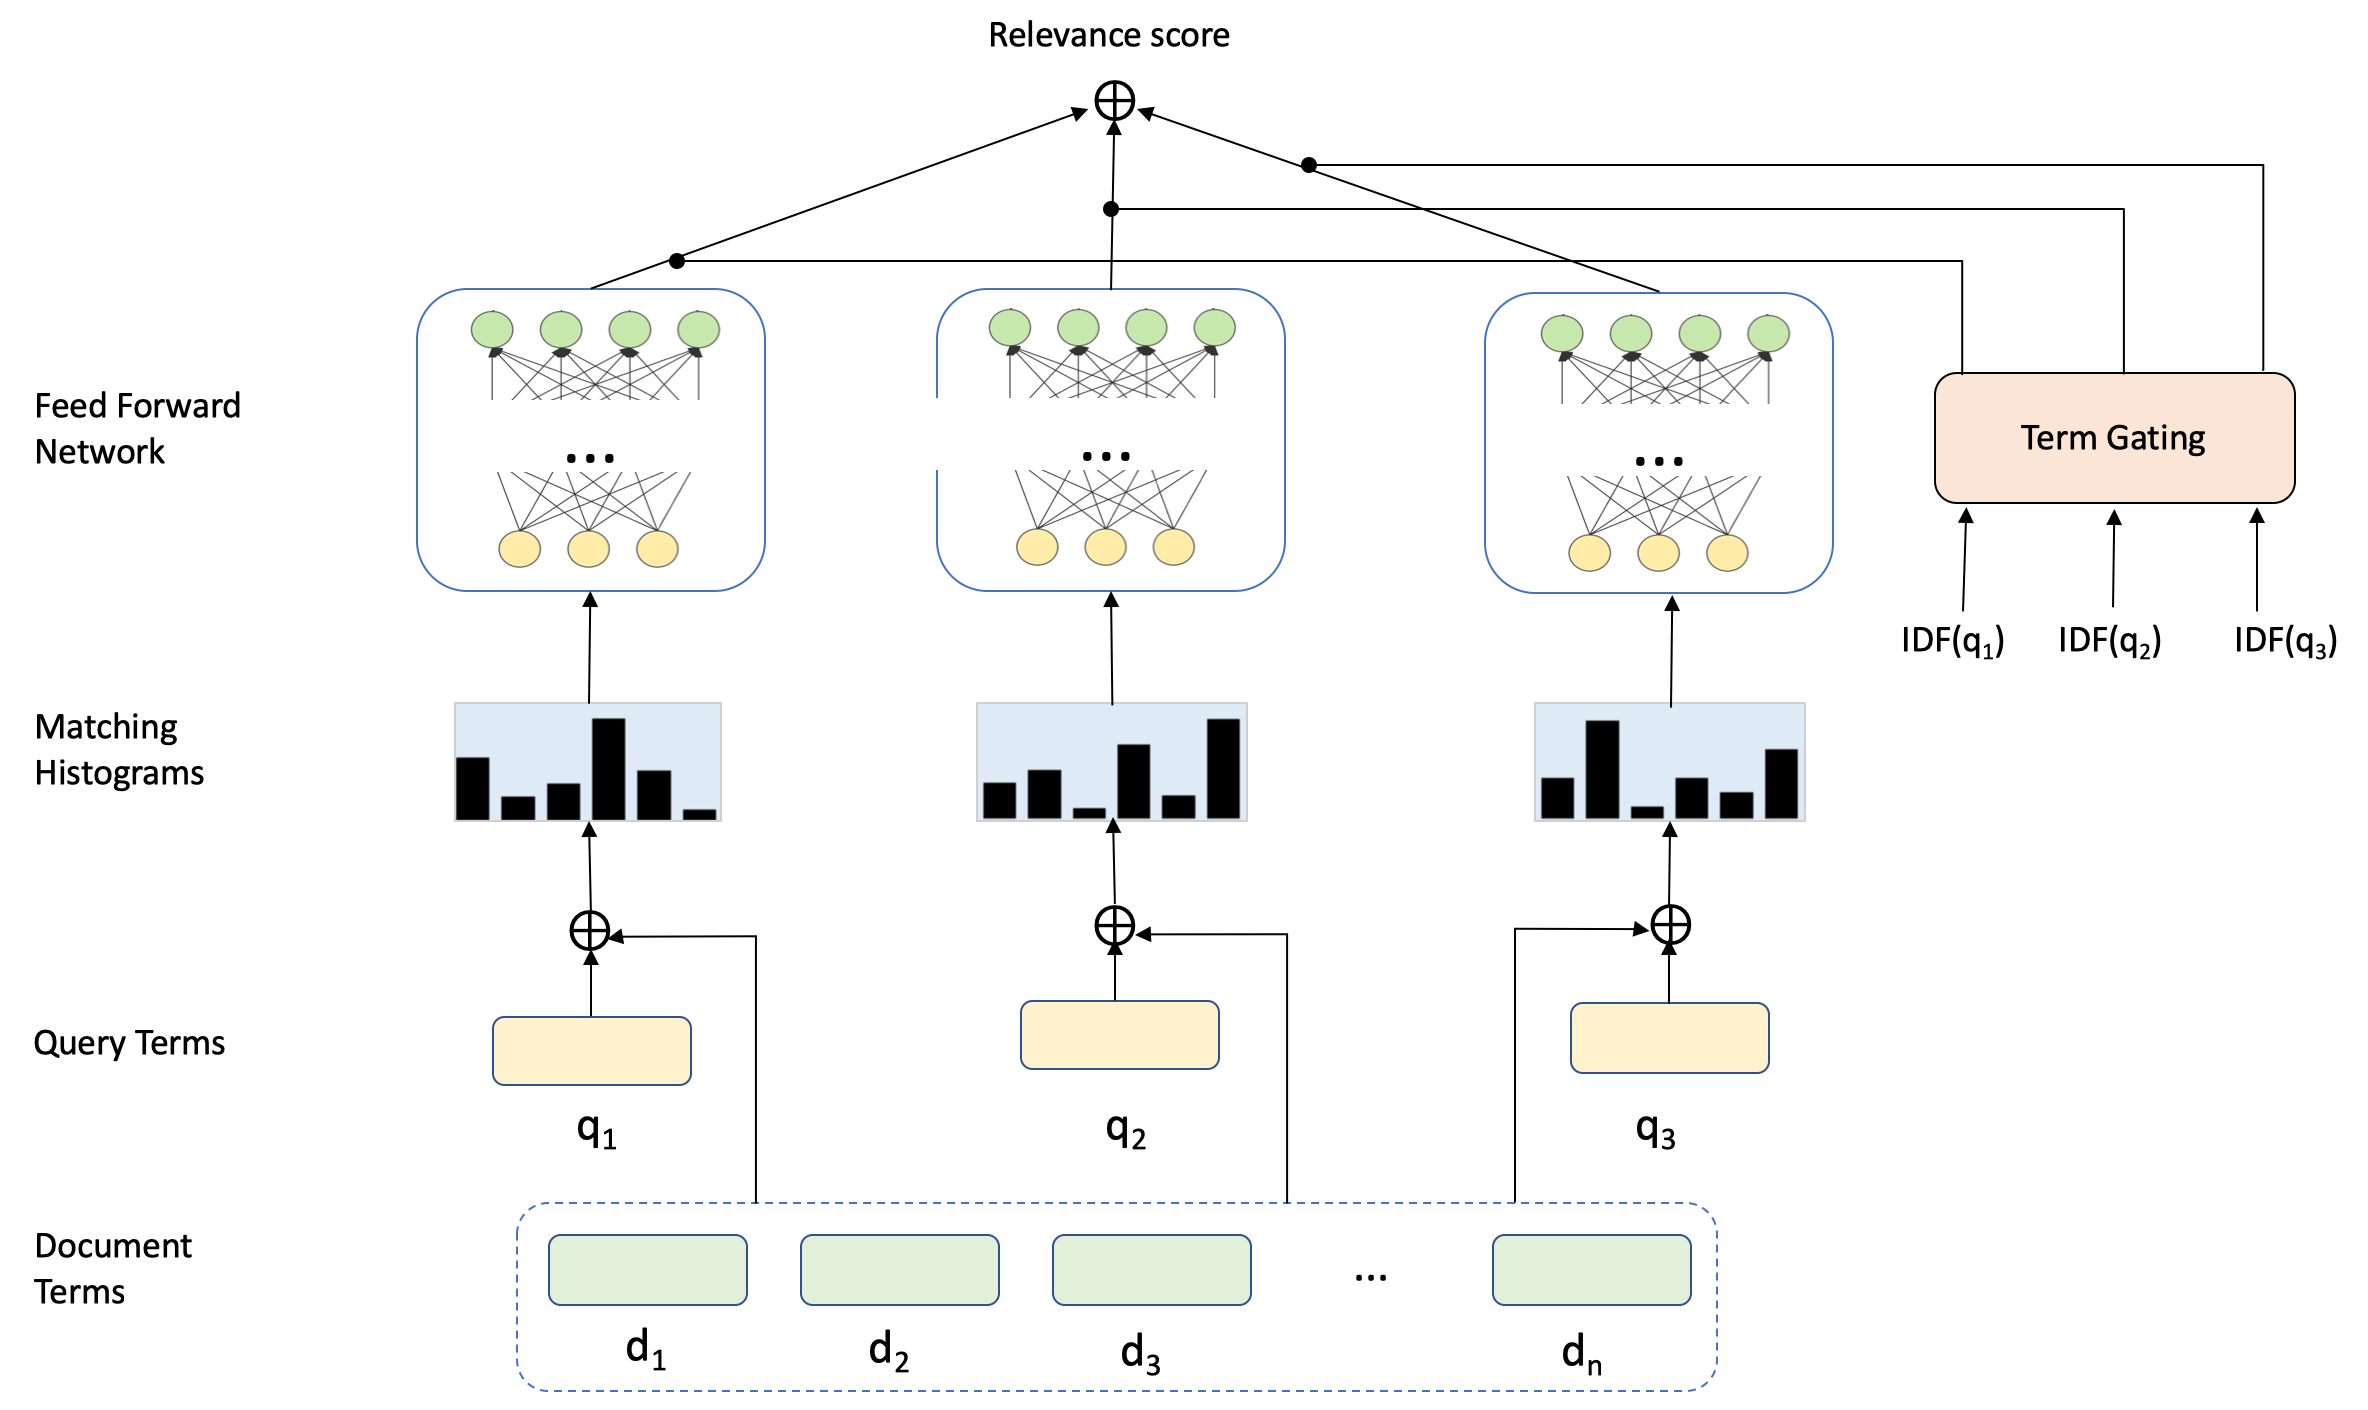
\includegraphics[width=15cm]{Figures/drmm_ppt.png}
    \caption{Deep Relevance Matching Model (DRMM) architecture}
    \label{fig:drrm_architecture}
\end{figure*}

Formally, both query and documents are represented using a set of term vectors denoted by $q=\{w^{(q)}_1,...,w^{(q)}_M\}$ and $d=\{w^{(d)}_1,...,w^{(d)}_N\}$, and $s$ denotes the final relevance score, then we have
\begin{align*}
    z^{(0)}_i &= h(w^{(q)}_i \otimes d), & i=1,....,M \\
    z^{(l)}_i &= \tanh(W^{(l)}z^{(l-1)}_i + b^{(l)}), & i=1,...,M,\ l=1,...,L \\
    s &= \sum_{i=1}^{M} g_i z^{(L)}_i &
\end{align*}
where $\otimes$ denotes the interaction operator (cosine similarity) between a query term and the document terms, $h$ is the mapping function to get matching histograms, $z^{(l)}_i$ denotes the intermediate hidden layers for the $i$-th query term, and $g_i$ denotes the aggregation weight from the term gating network.

\textbf{Matching Histogram Mapping}. Since the local interactions is within the interval [-1, 1], the histogram is obtained by discretizing the interval into a set of ordered bins and accumulating the count of local interactions for each bin. In this work, fixed size bins are used and the exact matching signal is treated as a separate bin. They explore three different ways of mapping:
\begin{description}
    \item[\normalfont\itshape Count-based Histogram (CH):] Takes the count of interactions in each bin as the histogram value.
    \item[\normalfont\itshape Normalized Histogram (NH):] Normalize the count value in each bin by the total count, to focus on relative rather than absolute number of different levels of interaction.
    \item[\normalfont\itshape LogCount-based Histogram (LCH):] Takes the logarithm over the count value in each bin, to reduce the range.
\end{description}

% \textbf{Feed forward Matching Network}. The matching histogram is used as input to a feed forward matching network to learn the hierarchical matching patterns and to produce a matching score for each query term. 

\textbf{Term Gating Network}. The model explicitly models query term importance using a term gating network to get a aggregation weight for each term. The softmax function is used as the gating function.
\begin{align*}
    \centering
    g_i &= \frac{\exp (w_g x^{(q)}_i)}{\sum_{j=1}^{M} \exp (w_g x^{(q)}_j)}, & i=1,...,M
\end{align*}
where $w_g$ is the weight vector of the gating network. Two different inputs were considered: \textit{term vector}, where query term vectors are used; \textit{inverse document frequency (IDF)}, where the IDF of the query term is used.

\textbf{Model Training}. The model is trained on triples ($q, d^+, d^-$), where document $d^+$ is ranked higher than document $d^-$ with respect to $q$, minimizing pairwise max-margin loss as in eq.~\ref{eq:drrm_loss_objective}.

\begin{equation}\label{eq:drrm_loss_objective}
    \mathcal{L}(q,d^+,d^-;\Theta) = \
    {\max (0, 1 - s(q,d^+) + s(q,d^-))}
\end{equation}
where $s(q,d)$ denotes the predicted matching score and $\Theta$ are the parameters of the feed forward network and term gating network. The stochastic gradient descent method \textsf{Adam} with mini-batches (20) is used to trained the model.

% \textbf{Datasets}. Experiments are run using two TREC collections Robust04 and ClueWeb-09-Cat-B. Topics are accumulated from TREC Web Tracks 2009, 2010, and 2011. ClueWeb-09-Cat-B is filtered to the set of documents with spam scores in the $60^{th}$ percentile, using the Waterloo fusion spam scores. For both datasets, both the title and description of the TREC topics are used. The retrieval experiments are conducted using the Galago search engine.

\subsection{Experimental Setup}\label{drmm_exp_setup}
We use the \textit{title} of each TREC topic as queries in our experiments. The indexing and retrieval is implemented using Lucene\footnote{\url{https://lucene.apache.org/}}. During indexing and retrieval, both document and query words are white-spaced tokenized, lower-cased and stemmed using Krovetz stemmer available here\footnote{\url{https://github.com/rmit-ir/KrovetzStemmer}}. Stopword removal is performed on the query words during retrieval from the Lucene index based on a custom stopwords list\footnote{See Lucene \textsf{EnglishAnalyzer} for details.}. We compare the DRMM model retrieval performance against the BM25 baseline using the default parameters (\textit{k1}:1.2 and \textit{b}:0.75) from Lucene.

%\paragraph{Term Embeddings}
\textbf{Term Embeddings}. The 300 dimensional vectors used as term embedding input for DRMM are trained using CBOW model~\citep{Mikolov2013} on Robust04 collection. The parameters used are context window size (10), negative samples (10) and subsampling of frequent words with a threshold of $10^{-4}$ using \texttt{word2vec}\footnote{\url{https://radimrehurek.com/gensim/models/word2vec.html}}. The corpus is preprocessed removing HTML tags, stemming using Krovetz stemmer and stopword removal using NLTK\footnote{\url{https://www.nltk.org/}}. We discarded from the vocabulary terms that occur less than 10 times in the collection resulting in a vocabulary of size 106K. The out-of-vocabulary (OOV) terms are ignored while preparing the model input.

\textbf{Model Implementation}. We implemented the DRMM model using the Keras functional api\footnote{\url{https://keras.io/getting-started/functional-api-guide/}} with a Tensorflow backend. The network configuration of the DRMM model is set as: one histogram layer (30 nodes), two hidden layers in the feed forward matching network (5 and 1 nodes) and 1 output layer with the term gating network for the final relevance score as suggested in the paper based on hyperparameter tuning on the validation set. We implement the variant DRMM\textsubscript{\textit{LCH}x\textit{IDF}} that uses \textit{logcount-based} histogram as input and \textit{term vector} for computing query term importance in the term gating network. We use a step-decay adaptive learning rate that drops the learning rate by a factor of 0.9 every 10 iterations (initial learning rate=0.001). We train the model for 100 iterations, where in each iteration the model trains on 1000 mini-batches (20). Thus, the model would train on roughly 2M training pairs of data. The training pairs for each mini-batch is randomly sampled from all possible pairs of relevant and irrelevant documents from the relevance judgements for the queries in the training set. 

\textbf{Evaluation}. We conduct 5 fold cross-validation to minimize overfitting due to the limited number of queries in the collection. Topics are randomly split into 5 folds and the parameters are tuned on 4-of-5 folds. The retrieval performance is evaluated on the final fold in each case using the optimal parameters. This process is repeated 5 times, once for each fold. Mean Average Precision (MAP) is the metric that is optimized for during training. We use a re-ranking strategy for evaluation, where first we retrieve the top-2000 documents using BM25 model and then re-rank it using the neural model to obtain the top-1000 documents that are used to compute the evaluation metrics. Each displayed metric is the average of the five 5-fold evaluation values.

\begin{table}[]
    \centering
    \begin{tabular}{lccc}
    \toprule
        Model Name & MAP & nDCG@20 & P@20 \\
        \midrule
        BM25 & 0.2405 & 0.4038 & 0.347 \\
        DRMM\textsubscript{\textit{LCH}x\textit{IDF}} & 0.257 & 0.4103 & 0.352 \\
        DRMM\textsubscript{\textit{LCH}x\textit{IDF}} \textit{paper} & 0.268 & 0.423 & 0.381\\
    \bottomrule
    \end{tabular}
    \caption{DRMM Model retrieval performance on the Robust04 collection}
    \label{tab:drmm_eval}
\end{table}

\subsection{Results and Discussion}
We observe from Table~\ref{tab:drmm_eval} that our implementation of DRMM provides improvements over the BM25 baseline across all evaluation metrics. However, this implementation gives results lower than that from the paper because of the following reasons: due to different random partitions of the data, and in the original paper they re-rank the top documents returned from a well-tuned query-likelihood (QL) model. Also, they use a different sampling strategy to generate the training pair instances since there is a data imbalance problem, where the pairs available for each query are significantly different (i.e. some queries have more positive samples than others). Then, the model could be dominated by a few queries leading to lower performance. 

We also empirically observe that using word embeddings not trained on the collection, such as, \texttt{word2vec}\footnote{\url{https://code.google.com/archive/p/word2vec/}} or \texttt{glove}\footnote{\url{https://nlp.stanford.edu/projects/glove/}} embeddings results in lower performance over the evaluation metrics. This is because the coverage of these term embeddings are only 35\% and 50\% of the 0.1M vocabulary using \texttt{word2vec} and \texttt{glove} respectively. The filtering of the vocabulary size from 0.6M to 0.1M by removing words that occur less than 10 times in the collection is a very important preprocessing step in effectively training a DRMM model that is better than the baseline. This is because there isn't sufficient data to learn reliable term embeddings for the words that occur less than 10 times in the collection. 

%-----------------------------------------------------
%	SECTION 2
%-----------------------------------------------------
\section{MatchPyramid for ad-hoc retrieval}

The MatchPyramid model for ad-hoc retrieval~\citep{matchpyramid16} is an interaction-focused model that first builds a matching matrix from the local interactions between the terms from query and document using word embeddings. 
%This model uses pretrained word embeddings to first create a query-document term interaction matrix, where each element is the cosine similarity between the query term and document term. 
This matching matrix is then viewed as an image and fed into a 2D convolutional neural network (CNN) to extract hierarchical matching patterns. Finally the matching patterns from the CNN are fed into a multi-layer perceptron (MLP) to aggregate a relevance score. The model is known to capture different matching patterns, such as, n-grams and un-ordered n-terms. The model architecture is shown in Figure~\ref{fig:matchpyramid_architecture}. %The `OOV' token is represented by an all-zeros embedding vector that is used for padding the input interaction matrix.
\begin{figure*}
    \centering
    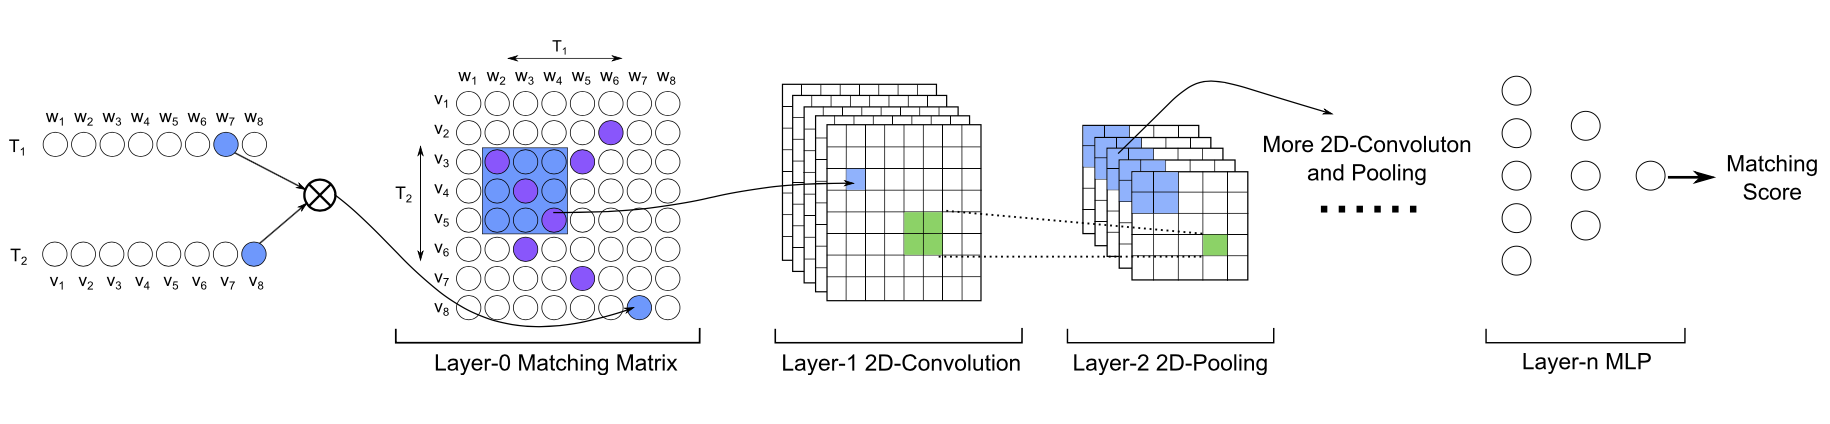
\includegraphics[width=\textwidth]{Figures/MATCHPYRAMID.png}
    \caption{MatchPyramid architecture~\citep{matchpyramid16}}
    \label{fig:matchpyramid_architecture}
\end{figure*}

\textbf{Matching Matrix}. It is a two-dimensional matrix where each element \textbf{M}\textsubscript{ij} denotes the similarity between the \textit{i}-th word $w_i$ in the query and the \textit{j}-th word $v_j$ in the document. The order in which the words appear is preserved while creating the matrix. They define four different similarity functions based on the words $w_i$ , $v_j$ or their corresponding embeddings: \textit{indicator function} (MP-Ind)--checks if two words are identical; \textit{cosine similarity} (MP-Cos)--between the word embeddings; \textit{dot product} (MP-Dot); \textit{gaussian kernel} (MP-Gau)--as defined in eq.~\ref{eq:mp_gau_kernel}.
\begin{equation}\label{eq:mp_gau_kernel}
    \mathbf{M}_{ij} = \
    e^{{-||\vec{w_i} - \vec{v_j}||}^{2}}
\end{equation}

\textbf{Hierarchical Convolution}. This consists of convolutional and dynamic pooling layers which are commonly used in CNN. The kernel sizes in each convolutional layer determines the maximum size of n-gram features that we take into account. And the pooling layer determines the most important information that needs to be selected from the convolutional layer. This is useful especially when we consider documents that have hundreds of words of which most are background words.

\textbf{Training Objective}. They use a pairwise ranking loss such as hinge loss with a margin of 1.0 for training the MatchPyramid model similar to the objective defined in eq.~\ref{eq:drrm_loss_objective} for the DRMM model.

\subsection{Experimental Setup}
The indexing and retrieval experimental setup for the TREC Robust04 collection is the same as described in section~\ref{drmm_exp_setup}. The term embeddings used for all the models are the \textit{glove} embeddings of 50 dimensions which are obtained by training on the Wikipedia corpus. We follow the exact same evaluation method as described for the DRMM model (section \ref{drmm_exp_setup}) here.

\textbf{Model Implementation}. We implement the model variants MP-Ind and MP-Cos using Keras. The optimization method \texttt{Adam} with mini-batches (32) is used for model training. The initial learning rate is set to $10^{-4}$ and uses a step-decay learning rate schedule that drops the learning rate by a factor of 0.9 after every 10 epochs. The network configurations for the MatchPyramid models are selected based on MAP on the validation set. We use one convolutional layer with kernel size 3 x 3 and feature maps set to 8, one dynamic pooling layer with pooling size 2 x 10, and two fully connected layers (128 nodes and 1 node respectively) with ReLU as the activation as suggested in~\citep{matchpyramid16}. We use one hierarchical convolution layer as more layers will lead to overfitting due to limited data. In our experiments, the maximum query length is set to 5 and the maximum document length is set to 500.

\begin{table}[]
    \centering
    \begin{tabular}{lccc}
    \toprule
        Model Name & MAP & nDCG@20 & P@20 \\
        \midrule
        BM25 & 0.2405 & 0.4038 & 0.347 \\
        MP-Ind & 0.1823 & 0.3353 & 0.286 \\
        MP-Ind \textit{paper} & 0.169 & 0.319 & 0.281 \\
        MP-Cos & 0.1898 & 0.3328 & 0.276\\
        MP-Cos \textit{paper} & 0.189 & 0.330 & 0.290\\
    \bottomrule
    \end{tabular}
    \caption{MatchPyramid models retrieval performance on the Robust04 collection}
    \label{tab:mp_eval}
\end{table}

\subsection{Results and Discussion}
When we look at Table~\ref{tab:mp_eval} we see that the MatchPyramid models cannot compete with the BM25 retrieval baseline across all measures. However, we can see that our implemented model performance is comparable to the model performance mentioned in the paper. As both MP-Ind and MP-Cos show similar performance, we can see that MP-Cos is able to encode exact matching along with semantic signals giving higher importance to exact matching over semantic similarities which is important for relevance matching. We empirically observe that it is better to use \texttt{glove} embeddings (50-dim) than the \texttt{word2vec} embeddings (300-dim) trained on the collection, this could be because the MatchPyramid models have a huge number of parameters and limited training data thus using an embedding with fewer (50) dimensions gives better performance. The best pooling size of 2 x 10 shows that it picks importance signals equivalent to the median query length on the query side, and on the document side, it aggregates importance signals from every 50 words which is close to the average length of a paragraph.

%------------------------------------------------------
%	SECTION 3
%------------------------------------------------------
\section{Deep Relevance Ranking using Enhanced Document-Query Interactions (PACRR-DRMM)}

In this paper~\citep{pacrr_drmm_18}, the focus is on enriching DRMM with context-sensitive representations of the query, as in the original model query terms are scored relative to the document terms without taking into consideration the context in which the term occurs, its akin to a Bag-of-Words (BoW) model. Whereas, the 
PACRR model~\citep{pacrr17,Yates17} is a \textit{position-aware} interaction based model that uses similarity matrices that captures semantic similarity between each query term and each individual term in the document, also preserving term order. Thus, PACRR-DRMM is an extension of DRMM, that uses the query term encodings obtained from PACRR-like convolutional \textit{n-gram} matching features as an input for the  DRMM model.

\textbf{PACRR}. The query-document similarity matrix (\textit{sim}) is created using the cosine similarity between the q-term and d-term embeddings. To keep the dimensions of the \textit{sim} fixed across queries and documents of varying length, the queries are padded to max query length $l_q$ and documents are either truncated/padded to max document length $l_d$\footnote{PACRR-\textit{firstk} as highlighted in~\citep{pacrr17}.}. Then the following pipeline is applied: 
\begin{description}[font=\normalfont\itshape]
    \item[convolutional relevance matching.]  convolutional layers of different kernel sizes $n$ x $n$ (n=2, 3,...,$l_g$) are applied on the similarity matrix to capture positional information over text windows of different lengths (\textit{n-grams}). For each kernel size, multiple kernel filters are used. The convolutional layer uses a stride (1, 1) along the query dimension and stride of (1, n) along the document dimension, so that it operates over consecutive terms that existed in the document.
    \item[max pooling layers.] First, max pooling is applied across the dimension of the filters to preserve the strongest signal from different filters. Then, row-wise \textit{k}-max pooling to capture the $k$ strongest signals for each query term and all document terms.
    \item[MLP for global relevance.] The resulting matrices are concatenated into a single matrix where each row is a document-aware query term encoding. To each row, the IDF of the query term is appended which is normalized by taking softmax with respect to the IDFs of all query terms. The rows are then concatenated to give a single vector that is used as input to a MLP~\citep{co_pacrr_wsdm18} to give a relevance score.
\end{description}

%These matrices are then fed through a series of convolutional, max-k pooling and recurrent layers to capture interactions, such as, bi-gram and tri-gram matches. In this model, convolutional layers are used to capture both unigram matching and positional information over text windows over different lengths; max-k pooling layers are along query dimension, to preserve matching signals across different query terms; recurrent layer combines signals from different query terms to produce query-document relevance score.

%The similarity between a query term and document term is calculated by taking the cosine similarity between the corresponding pre-trained word2vec vectors. Query-document similarity matrices can provide rich signals to perform n-gram matching which corresponds to consecutive document terms that are highly similar to at least one of the query terms. Since the subsequent processing in PACRR's convolutional layer requires that each query-document similarity matrix have the same dimensions, we transform the raw similarity matrices $sim_{|q|*|d|}$ to $sim_{l_q * l_d}$ matrices with uniform number of rows and columns. The query dimension $l_q$ is zero padded to the maximum query length. Two strategies were designed with respect to the document dimension $l_d$.
% \begin{itemize}
%     \item \textit{firstk} - In this the first $k$ columns/terms of the matrix are kept. If $k > |d|$ then the remaining columns are zero-padded.
%     \item \textit{kwindow} - For the case of unigrams, the top $l_d$ terms with the highest similarity to query terms are chosen. But for text snippets of length $n$, a similarity matrix $sim^n_{l_q * l_d}$ is created for each query-document pair and $n$. So $kwindow$ calculates the maximum similarity between each term in $n$ and the query terms, and then calculates the average similarity over each $n$-term window. Then the top $k$ windows based on the average similarity is selected.
% \end{itemize}

% \textbf{Convolutional relevance matching} is to match text snippets with different length from a query and a document given an query-document similarity matrix as input. Each convolutional layer is responsible for a specific n: by applying a kernel to $n * n$ windows, providing a similarity signal for each window. When \textit{firstk} method is used, each convolutional layer gets the same similarity input matrix $sim_{l_q * l_d}$ because \textit{firstk} produces same matrix irrespective of $n$. But when $kwindow$ method is applied each convolutional layer will get a similarity matrix $sim^n_{l_q * l_d}$ corresponding to the kernel $n * n$. Different convolutional layers with kernel sizes $2*2, 3*3,....,l_g*l_g$ corresponding to bi-gram, tri-gram and n-gram matchings are used. Each convolutional layer applies $n_f$ filters, $n_f$ is a hyperparameter. The convolutional layer uses a stride (1,1) along the query dimension and stride of (1,n) along the document dimension, so that it operates over consecutive terms that existed in the document.

% \textbf{Two max pooling layers} is to capture the strongest similarity signals for each query term. A small number of signals $n_s$ is used so that the model is not biased by document length. For each query term, first max-pooling is performed over the filter dimension $n_f$ to keep the strongest indicator from the different filters, as they assume that there is only a single true matching in a $n*n$ window. Then $k-max$ pooling is performed over the query dimension to keep the $n_s$ strongest signal for each query, thus producing a 3-dimension tensor $P_{l_q * l_g * n_s}$.

% \textbf{Recurrent layer for global relevance} is to transform the query term similarity signals in $P_{l_q * l_g * n_s}$ into a document relevance score. A Long Short-Term Memory (LSTM) recurrent layer is applied to $P$, taking a sequence of vectors as input and transforming it to a final relevance score. After splitting the above matrix across the query dimension, then for each query $q_i$ we have a matrix $P_{l_g*n_s}$ which is flattened into a vector by concatenating rows together and appending the normalized IDF score of $q_i$.

\begin{figure*}
    \centering
    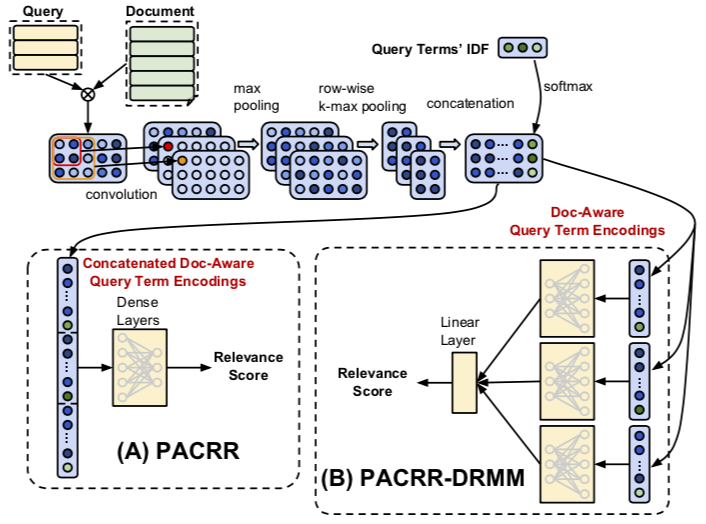
\includegraphics[width=10cm]{Figures/pacrr_drmm.png}
    \caption{PACRR-DRMM architecture~\citep{pacrr_drmm_18}}
    \label{fig:pacrr_drmm_pipeline}
\end{figure*}

\textbf{PACRR-DRMM}. In this version of the PACRR model, instead of using a MLP to score the \textit{concatenation} of all document-aware q-term encodings, the MLP is used independently to score each q-term encoding similar to DRMM and then the resulting scores are aggregated using a linear layer. The architecture of the model along with its comparison to the PACRR model can be seen in Figure~\ref{fig:pacrr_drmm_pipeline}. The scores of the q-terms from MLP is not weighted using a \textit{gating} mechanism like in DRMM, however since the IDF of q-term is appended to the encoding are a form of term-gating.


\textbf{Training objective}. The model (fig.~\ref{fig:pacrr_drmm_pipeline}) is trained by minimizing the cross entropy loss as defined in eq.~\ref{eq:pacrr_loss_objective} as it has been demonstrated to give better results~\citep{Dehghani_sigir17}.
\begin{equation}\label{eq:pacrr_loss_objective}
    \mathcal{L}(q,d^+,d^-;\Theta) = \
    -log\frac{exp(rel(q,d^+))}{exp(rel(q,d^+)) + exp(rel(q,d^-))}
    %{\max (0, 1 - rel(q,d^+) + rel(q,d^-))}
\end{equation}

\subsection{Experimental Setup}
The indexing and retrieval experimental setup for the TREC Robust04 collection follows as described in section~\ref{drmm_exp_setup}. The same evaluation method as described for the DRMM model (\ref{drmm_exp_setup}) is implemented here.

\textbf{Input Preprocessing}. The document and query words are white-spaced tokenized, lower-cased and stemmed using Krovetz stemmer. But no stopword removal is applied on the texts. Thus, the vocabulary size is 0.3M which is bigger than that considered for both DRMM and MatchPyramid (0.1M). 

\textbf{Term Embeddings}. This model uses 200-dimension \texttt{word2vec} embeddings trained on the collection with negative sampling and window size set to 5 and the rest of the hyperparameters set to default\footnote{\url{https://radimrehurek.com/gensim/models/word2vec.html}}. The word embeddings are not updated while training the PACRR-DRMM model. The OOV term is represented with an embedding that is the average of all the term embeddings in the vocabulary.

\textbf{Model Implementation}. The model is implemented in Keras with TensorFlow backend. It is trained using the \texttt{Adam} optimization method with learning rate of 0.001 and mini-batches (32) that contains randomly sampled irrelevant document for each relevant document found in the top-1000 BM25 retrieved results for each query. The training usually converges within 50 epochs, with the weights uniformly initialized. The irrelevant documents are also sampled from the top-1000 BM25 documents which are not marked as relevant. We follow the network configuration as specified in Appendix A of the paper. The maximum query length $l_q$ is set to 5 and maximum document length $l_d$ to 1000. The maximum kernel size ($l_g$ x $l_g$) for the convolutional layers is set to (3 x 3) with number of filters equal to 16. For row-wise \textit{k}-max pooling, $k$=2. A two layer MLP with ReLU activations and hidden layers with 7 nodes to score each document-aware q-term encoding. Finally, the scores of each document-aware q-term encoding are aggregated using a linear layer (1 node MLP). 

\subsection{Results and Discussion}
\begin{table}[]
    \centering
    \begin{tabular}{lccc}
    \toprule
        Model Name & MAP & nDCG@20 & P@20 \\
        \midrule
        BM25 & 0.2405 & 0.4038 & 0.347 \\
        PACRR & 0.260 & 0.442 & 0.372\\
        PACRR-DRMM & 0.263 & 0.445 & 0.374 \\
        PACRR-DRMM \textit{paper} & 0.259 & 0.444 & 0.373 \\
    \bottomrule
    \end{tabular}
    \caption{PACRR-DRMM model retrieval performance on the Robust04 collection}
    \label{tab:pacrr_drmm_eval}
\end{table}
From Table~\ref{tab:pacrr_drmm_eval}, we see that both PACRR and PACRR-DRMM shows improvements over the BM25 baseline across all evaluation metrics. We also see that the model trained using the architecture configuration mentioned above, gives a retrieval performance that is quite close to the model trained in the paper across all the metrics. This is because we used the same partitions\footnote{\url{https://archive.org/download/deep_relevance_ranking_data/robust04_data.tar.gz}} of the topics shared by the authors that was used for cross-validation along with the pre-processed documents (``HTML" tags removed) for each fold, the top-k documents retrieved from BM25 using Galago\footnote{\url{http://www.lemurproject.org/galago.php}} and the pre-trained word embeddings. We observe that PACRR-DRMM performs slightly better than PACRR, this is likely due to the fewer parameters of the MLP layer which is shared between all q-term encodings and as it uses a shorter input representation.
%-----------------------------------
%	SUBSECTION 2
%-----------------------------------

% \subsection{CO-PACRR}

% \begin{figure*}
%     \centering
%     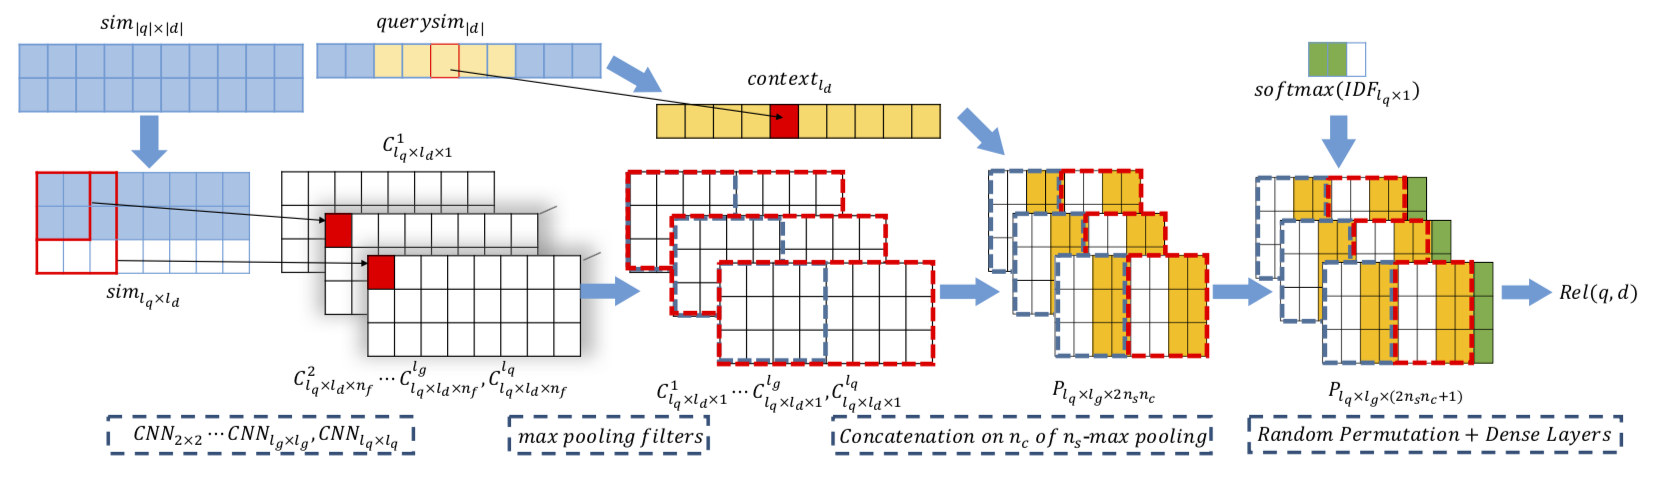
\includegraphics[width=\textwidth]{Figures/COPACRR.png}
%     \caption{CO-PACRR pipeline}
%     \label{fig:co_pacrr_pipeline}
% \end{figure*}

\section{Neural Pseudo-Relevance Feedback (NPRF-DRMM)}
\label{sec:nprf_drmm_reproducibility_desc}
In this work~\citep{li2018nprf}, they proposed a generic neural pseudo relevance feedback framework (NPRF) that helps the application of PRF with existing neural IR models (NIRM). For a given query and target document, NPRF produces a final relevance score by considering the interactions of the target document with the query as well as the top-$n$ feedback documents from the initial ranking (e.g. BM25, QL). The proposed framework directly incorporates existing neural IR models without the need to modify their architectures as shown in Figure~\ref{fig:nprf_drmm_pipeline}.

% \textbf{Initial ranking}. An initial ranking $rel_q(q, d)$ is applied to obtain the top-$n$ documents denoted as $D_q$ for $q$.

\textbf{Extracting document interactions}. Given the target document $d$ and each feedback document $d_q\in D_q$, $rel_d(d_q, d)$ is a NIRM that is used to compute the $n$ relevance scores. Since DRMM takes as input matching histograms (\textit{LCH}x\textit{IDF}) from the cosine similarity between pairs of term embeddings from $d$ and $d_q$ without considering term dependencies, so $d_q$ is summarized by keeping the top-$k$ terms based on \textit{tf-idf} scores to remove noisy or irrelevant terms.

\begin{figure*}
    \centering
    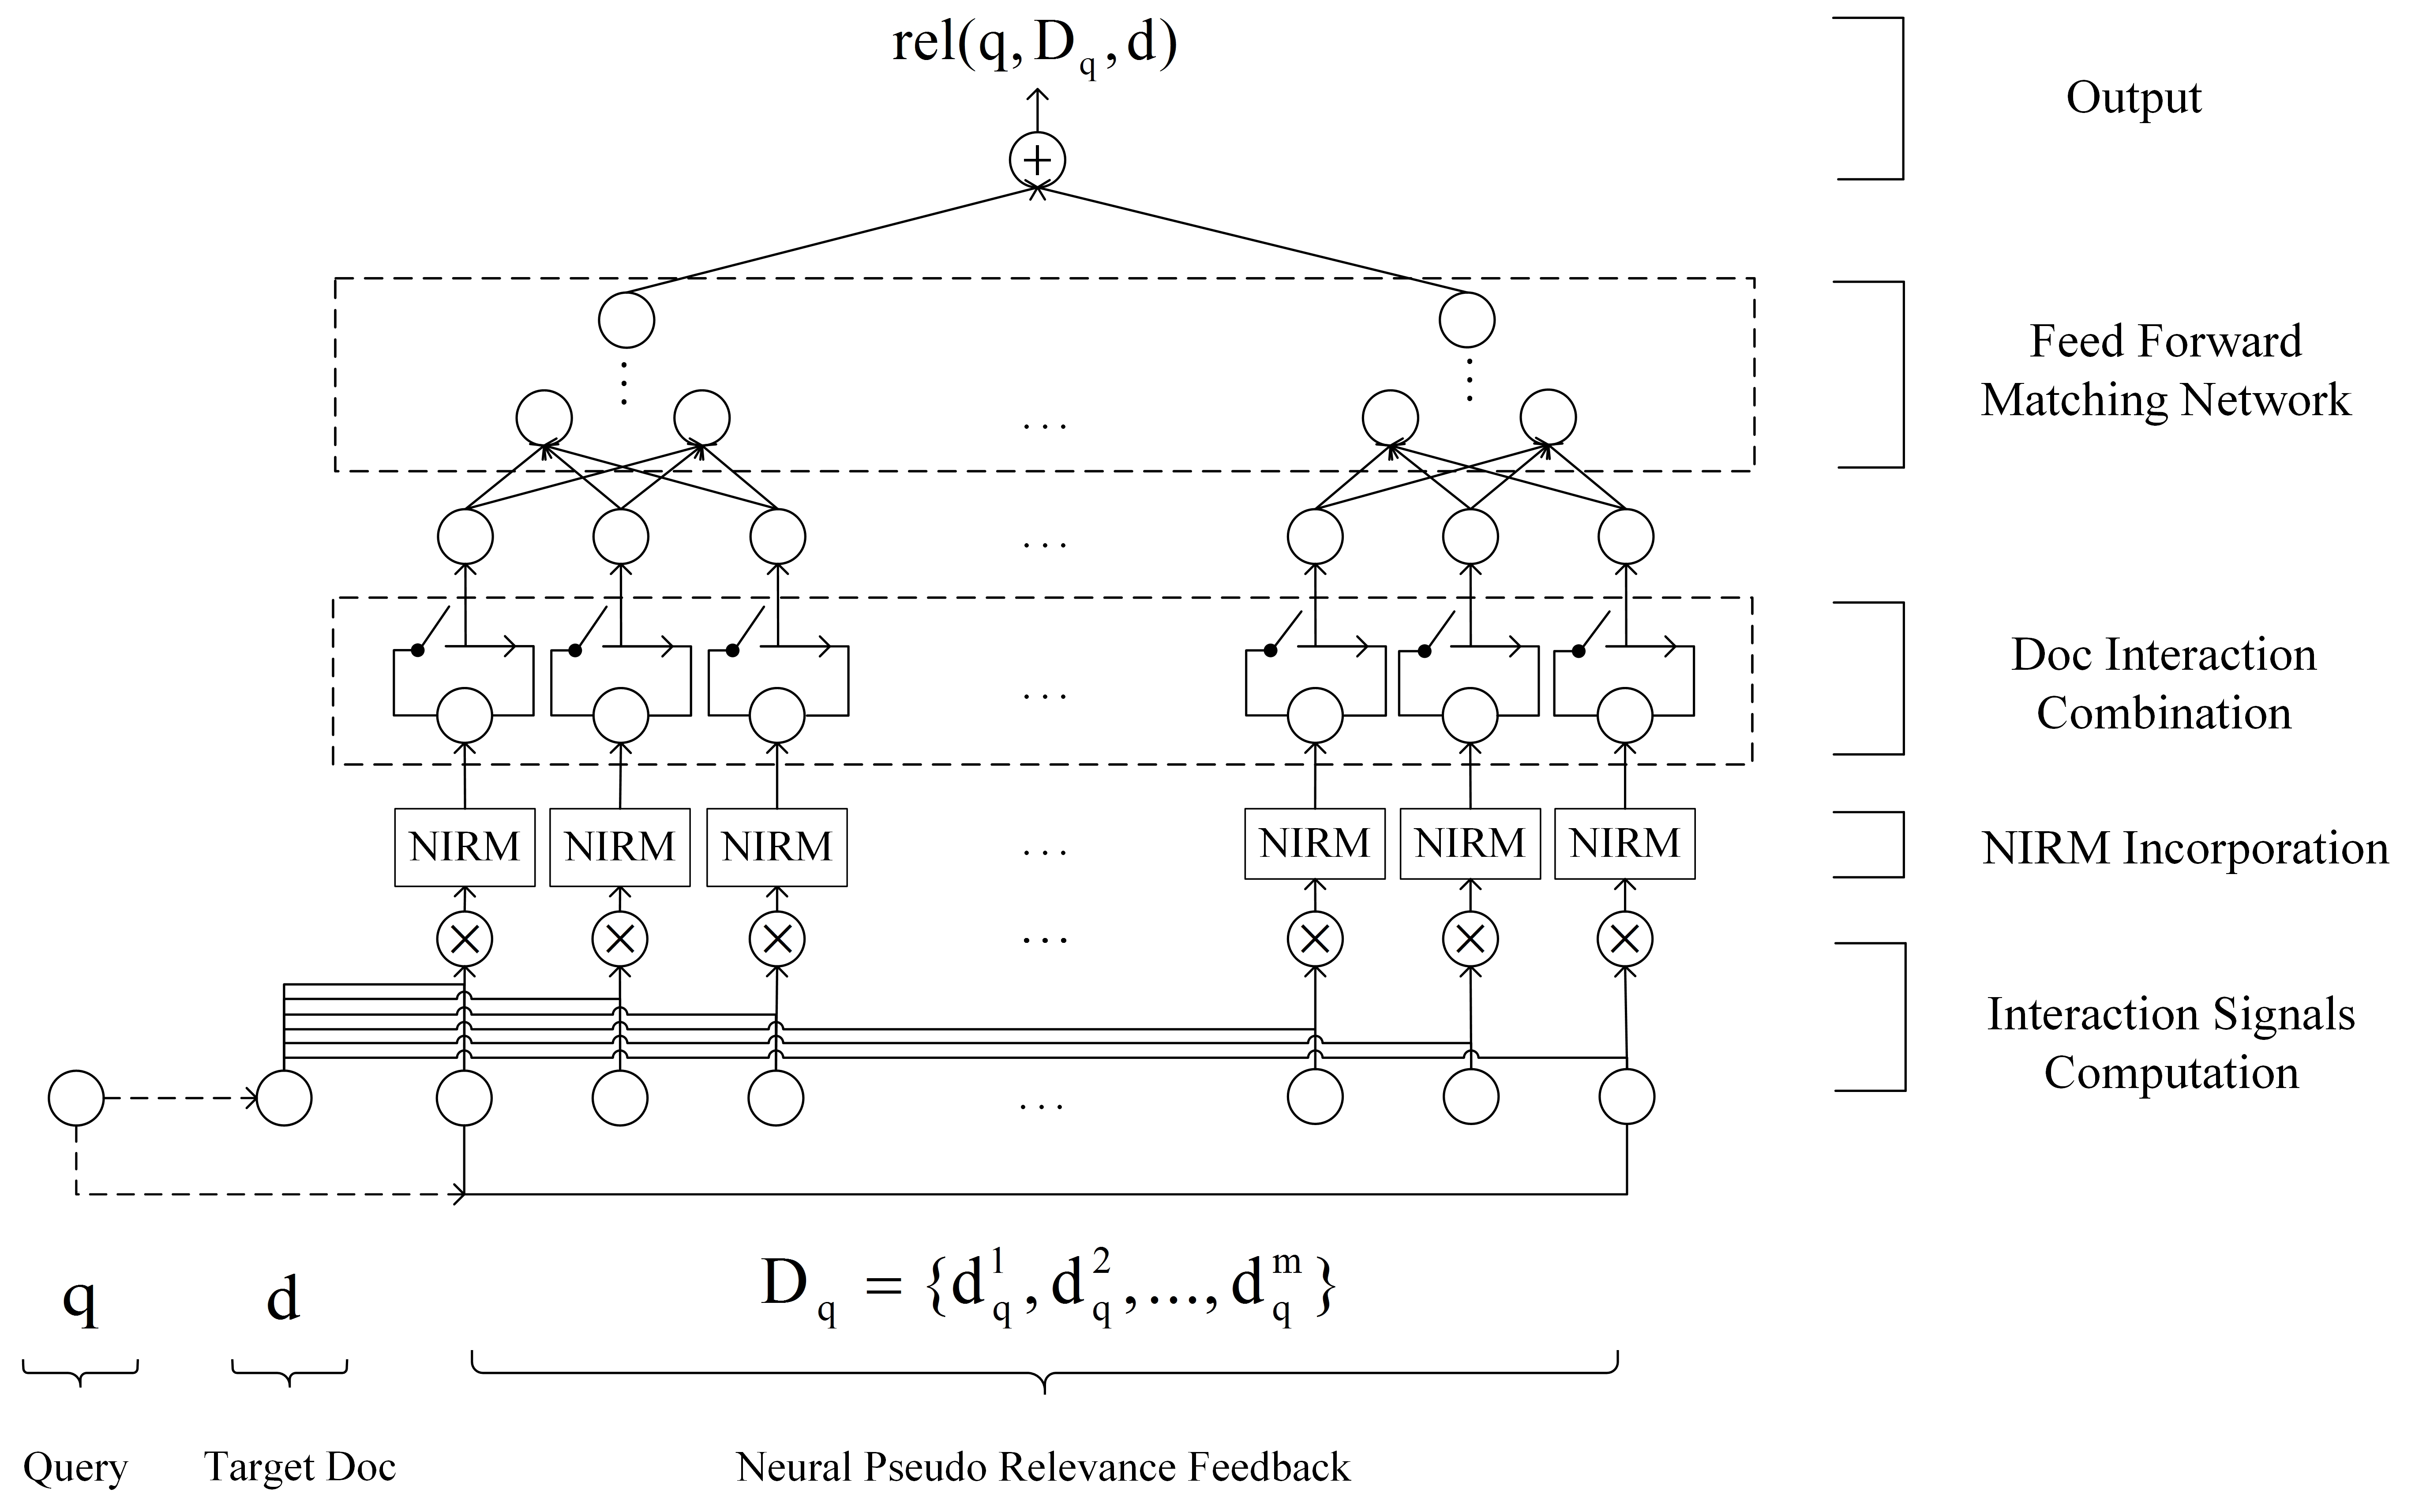
\includegraphics[width=14cm]{Figures/NPRF-arch.jpg}
    \caption{Neuro Pseudo Relevance Framework (NPRF) architecture~\citep{li2018nprf}}
    \label{fig:nprf_drmm_pipeline}
\end{figure*}

\textbf{Combining document interactions}. When combing the relevance scores for the feedback documents, the relevance of $d$ from the initial ranking $rel_q(q, d_q)$ is also important. Thus, weighted relevance document score $rel_d'(d_q, d)$ is computed using the equation~\ref{nprf_doc_rel} with min-max normalized $rel_q(q, d_q)$ score.
\begin{equation}\label{nprf_doc_rel}
    rel_{d}'(d_q, d) = rel_d(d_q, d)(0.5 + 0.5 * rel_q(q, d_q))
\end{equation}
The $rel_d'(d_q, d)$ of each $d_q \in D_q$ is combined into a single relevance score using two variants: (i) direct summation, and (ii) using feed forward network with \textit{tanh} activations.

\textbf{Training Objective}. A pairwise ranking loss such as hinge loss with a margin of 1.0 is used for training the model similar to the objective defined in eq.~\ref{eq:drrm_loss_objective}.

\subsection{Experimental Setup}
\label{sec:nprf_drmm_reproducibility_exp}

The indexing and retrieval experimental setup for the TREC Robust04 collection is the same as described in section~\ref{drmm_exp_setup}. The term embeddings used are the \texttt{word2vec} embeddings of 300 dimensions trained on the Robust04 collection using the setup described in section~\ref{drmm_exp_setup}. Akin to the evaluation setup for DRMM described in section~\ref{drmm_exp_setup}, the proposed NPRF\textsubscript{ds}-DRMM model is used to re-rank the top-2000 documents retrieved from BM25 and uses the same 5-fold cross validation setup to measure the model's retrieval performance.

\textbf{Model Implementation}. The model implemented in Keras is trained using the \texttt{Adam} optimizer with a batch size of 20 and an initial learning rate of $10^{-3}$ followed by step-decay learning rate schedule that drops the rate by a factor of 0.9 after every 25 iterations. Usually, the training converges within 30 epochs or maximum 250 iterations (on each iteration the model trains on 100 mini-batches). The variant that we implemented is NPRF\textsubscript{ds}-DRMM that is based on the direct summation of the weighted feedback document relevance scores as that was shown to have the best performance across all the variants~\citep{li2018nprf} on the TREC Robust04 collection. The top-10 documents from BM25 are used as the pseudo relevant feedback document input $D_q$ for the model, where each $d_q \in D_q$ is summarized by the top-20 terms based on \textit{tf-idf}. The network configuration for the DRMM component is using the DRMM\textsubscript{\textit{LCH}x\textit{IDF}} variant with the original configuration (\citep{Guo2016}) that includes a histogram input layer of 30 nodes, two hidden layers in MLP (5 and 1 node respectively), and one output node with term gating (\textit{IDF}-softmax values) for the feedback document relevance score. A different sampling strategy is used to generate the training pair instances that takes into consideration the data imbalance problem thus generating about the same number of pairs across all the queries even if some queries have more positive samples than others\footnote{\url{https://github.com/ucasir/NPRF/blob/master/utils/pair_generator.py\#L100}}.

\subsection{Results and Discussion}
\begin{table}[]
    \centering
    \begin{tabular}{lccc}
    \toprule
        Model Name & MAP & nDCG@20 & P@20 \\
        \midrule
        BM25 & 0.2405 & 0.4038 & 0.347 \\
        %PACRR & 0.260 & 0.442 & 0.372\\
        NPRF\textsubscript{ds}-DRMM & 0.2869 & 0.4585 & 0.4006 \\
        NPRF\textsubscript{ds}-DRMM \textit{paper} & 0.2904 & 0.4502 & 0.4064 \\
    \bottomrule
    \end{tabular}
    \caption{NPRF-DRMM model retrieval performance on the Robust04 collection}
    \label{tab:nprf_drmm_eval}
\end{table}
From Table~\ref{tab:nprf_drmm_eval}, we see that NPRF\textsubscript{ds}-DRMM shows significant improvements over the BM25 baseline across all evaluation metrics. We also see that the model trained using the architecture configuration mentioned above, gives a retrieval performance that is quite close to the model trained in the paper across all the metrics. This is because we used the same partitions of the topics shared by the authors as part of the code\footnote{\url{https://github.com/ucasir/NPRF/blob/master/model/nprf_drmm_config.py}}. The small differences in the metrics is because the preprocessing that we used is different from that mentioned in the paper where they used a porter stemmer instead of krovetz stemmer and also the word embeddings are trained differently by using the pool of top-2000 documents returned from BM25 for each individual queries as suggested by~\cite{diaz16} instead of the entire Robust04 collection as we used in section~\ref{drmm_exp_setup}.

%-----------------------------------------------------
%	SECTION 5
%-----------------------------------------------------
\section{Deep Structured Semantic Models (DSSM)}
The Deep Structured Semantic Model (DSSM)~\citep{dssm13} is based on Siamese networks used for short text matching. The model is trained on pairs of query and documents titles, both texts represented as a bags-of-character-trigraphs. This architecture consists of two deep models--for the query as well as the document--with fully-connected layers and cosine distance as the similarity function. They train the model on clickthrough data where each sample consists of a query \textit{q}, positive documents $d^{+}$ (document clicked by user on SERP page) and a set of negative documents $D^{-}$ randomly sampled uniformly from the collection. The model is trained by minimizing the cross-entropy loss after taking a softmax over the model outputs for all the candidate documents,
\begin{equation}
\begin{split}
	\mathcal{L}_{DSSM}(q,d^+,D^-) = \
    {\log (\frac{e^{\gamma \cdot \cos (\vec{q},\vec{d^+})}}{\sum_{d \in D}e^{\gamma \cdot \cos (\vec{q},\vec{d})}})} \\
    where, D = {d^+} \cup D^-
\end{split}    
\end{equation}
\begin{figure}
    \centering
    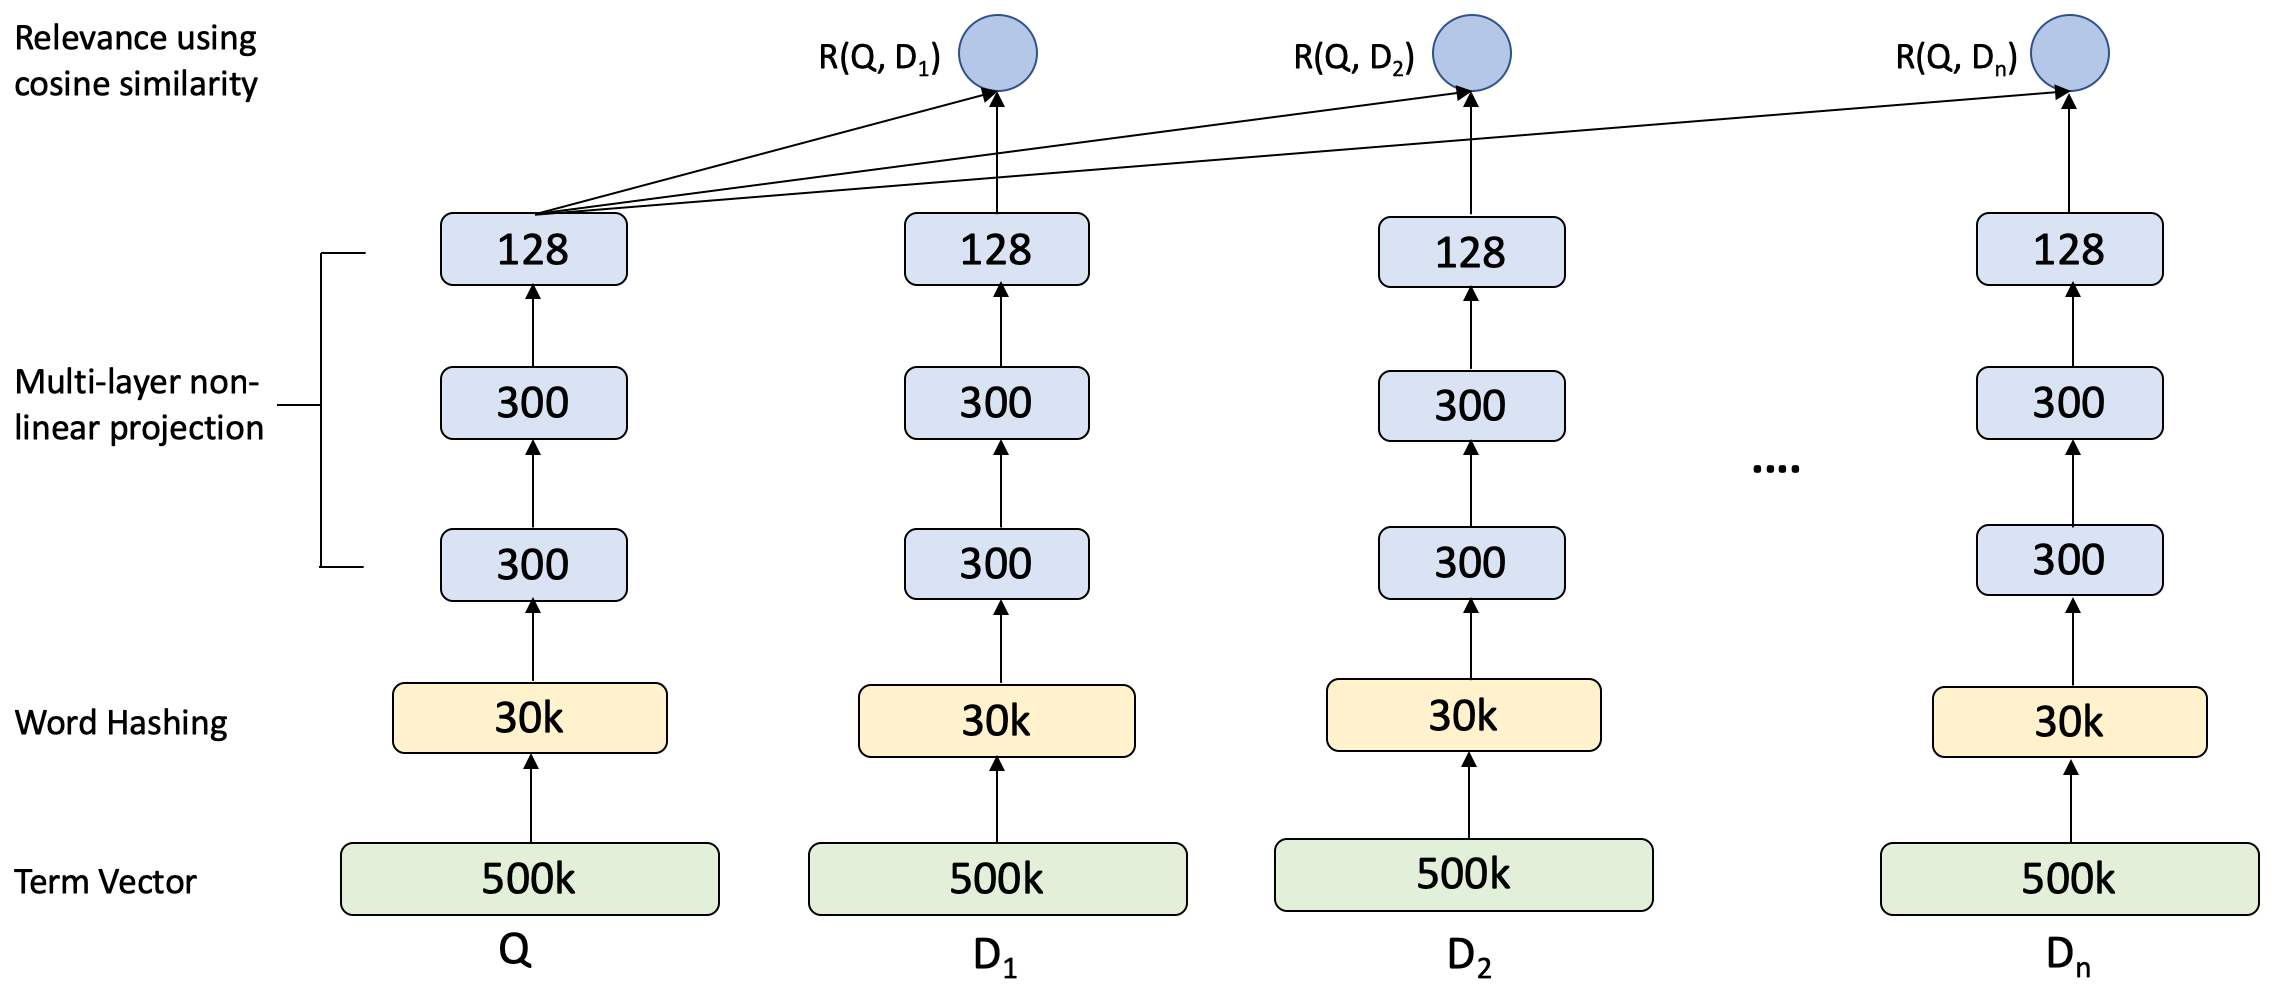
\includegraphics[width=12cm]{Figures/dssm_ppt.png}
    \caption{Deep Structured Semantic Model (DSSM) architecture
    %The first hidden layer with 30k units, accomplishes word hashing. The word-hashed features are then projected through multiple layers of non-linear projections. The final layer output produces the low-dimensional dense vector in the semantic space.
    }
    \label{fig:dssm_architecture}
\end{figure}

\subsection{Experimental Setup}
The indexing and retrieval experimental setup for the TREC Robust04 collection is the same as described in Section~\ref{drmm_exp_setup}. Since DSSM needs large scale training data (large click-through dataset), due to its huge parameter size, we try to train the model using two strategies: pretraining the triletter embeddings using the Robust04 collection instead of training it during model training, and using weak supervision to train the model with AOL query logs as suggested by~\cite{Dehghani_sigir17}. The models implemented in Keras are trained using the \texttt{Adam} optimizer with varying batch sizes and learning rates. The parameters of the DNN is shown in Figure~\ref{fig:dssm_architecture}, the only difference is that the number of nodes in the word hashing layer depends on the triletters obtained from the Robust04 collection.

\subsubsection{Pretraining Triletter Embeddings}

The input for the DSSM model is the bag-of-character triletter vector which is of much lower dimensionality ($\sim$15k) than term vectors which are usually the size of the vocabulary ($\sim$500k), thus enabling us to effectively train a deep neural network (DNN). Due to the limited number of queries and smaller size of the training dataset from Robust04 collection in comparison to the Bing Web collection that is used in the paper, we first train the triletter embeddings from the collection so that the limited training data can then be used to effectively learn dense representations for both queries and documents.

The 300 dimensional triletter embeddings are trained using the skip-gram model with negative sampling (SGNS)~\citep{Mikolov2013}. The corpus is preprocessed removing HTML tags, but no stemming and stopword removal is applied. Each word (e.g. \textit{good}) in the collection is first represented with starting and ending marks (e.g. \textit{\#good\#}) after which they are split into triletter \textit{n-grams} (e.g. \textit{\#go, goo, ood, od\#}). The corpus then comprises of documents represented using the triletters instead of words which are then used to train the embeddings. The parameters used are context window size (5), negative samples (10), minimum triletter frequency (5) and subsampling of frequent words with a threshold of $10^{-4}$ using \texttt{word2vec}\footnote{\url{https://radimrehurek.com/gensim/models/word2vec.html}} (\texttt{sg=1} and \texttt{hs=0}). The model is trained for 20 epochs over the corpus. The parameters for the model were chosen based on~\cite{ngram_embeddings17}, where they describe how to compute word embeddings by training \textit{n-gram} embeddings and then representing each word by the sum of these representations.

\subsubsection{Weak supervision with AOL query logs}

\textbf{Training query set}. We prepare the training query set using the setup described in~\cite{Dehghani_sigir17}, which comprises of unique queries that appear in the AOL query logs. We filter out navigational queries containing URL substrings (``http'',``www.'', ``.com'', ``.net'',``.org'', ``.edu''). All non-alphanumeric characters from the queries were removed. All queries that are present in the evaluation Robust04 queries are removed from the training set. Finally, only those queries that have at-least 10 documents retrieved by BM25 from Robust04 are kept, thus giving us a set of 6.15 million queries are after preprocessing. We also created smaller subsets of queries (1k, 10k) to see if we can effectively train a small model and 1M as that should already give us sufficient data to train the model.

\textbf{Training data}. In~\cite{Dehghani_sigir17}, they retrieve the top-1000 documents using BM25 for each query in the training query set and generate $|Q|$x$1000^2$ ($\sim$6E13) pairwise training pairs. Due to limited computational resources and time, we used different sampling strategies to generate the pairs:
\begin{itemize}
    \item For each positive document that we consider from the top-10, we sample 4 negative documents from the rest of the top-1000 documents.
    \item For each positive document from the top-10, we sample 3 negative documents randomly from the rest of the collection and 1 negative document from the rest of the top-1000 based on probability distribution over the BM25 scores.
    \item For each positive document from top-10, we sample 4 negative documents from the rest of the collection.
    \item For a positive document from top-1, we randomly sample 4 negative documents from the rest of the collection.
\end{itemize}

\textbf{Document text}. In the DSSM paper, they train the model on query-document title pairs where title is extracted from the title field from the index. Thus, we also tried training the model on different document text versions since the Robust04 collection doesn't have a specific title field in many of the documents ($\sim$65\%)-- full-text of document, the first 3 sentences of the document as the title, the first 2 sentences as the title and the first 3 sentences plus the snippet as title for the positive documents.

\subsection{Results and Discussion}

Using the various strategies described above to train the DSSM model, we couldn't effectively train a model that performs better than BM25 baseline\footnote{\url{https://www.comet.ml/neural-ir/dssm-weak-supervision}}. The poor effectiveness of the DSSM model (\textit{representation-focused}) is also highlighted in previous studies~\citep{Guo2016, matchpyramid16}. One possible reason for the poor effectiveness is that it is difficult to learn a good global representation of the documents in the Robust04 collection to match with the representation learnt for a related query.

However, these results are inconsistent with that of~\cite{Dehghani_sigir17} where they show a model based on representation learning and weakly supervised with BM25, gives a performance better than BM25. Our results with weak supervision reflects the same performance as in this study~\citep{Nie_ictir18}, where they hypothesize that the difference in performance could be due to the huge difference in computation resources where they train a very large number of training pairs ($\sim$6E13) for a large number of epochs. One other reason could be that the size of the dense input representation has a much smaller dimensionality (300-dimension normalized weighted element-wise summation of the term embeddings) whereas for DSSM it is about 15k.

% \clearpage
\section{Performance Comparison of Trained Models}
\label{sec:compare_perform_trained models}
In this section, we briefly compare the retrieval performance of the implemented neural retrieval models as seen in Table~\ref{tab:comparison_all_model_eval}. We can see that all of the implemented neural retrieval models perform better than the traditional BM25 baseline as highlighted in previous work, except for MatchPyramid which is similar to the conclusion they get in the original paper~\citep{matchpyramid16}. 

We can clearly observe that \textit{position-aware} neural IR models, like, PACRR and PACRR-DRMM that takes into consideration the context of the query terms perform better than DRMM which computes the interactions between the query and document terms ignoring the context. Also, we see that the NPRF model (NPRF\textsubscript{ds}-DRMM) which incorporates pseudo relevance feedback into the existing DRMM model, improves on the DRMM retrieval performance across all evaluation metrics. We also provide a comparison of the hyper-parameters between the implemented neural retrieval models in Table~\ref{tab:hyperparam_all_models}.

\begin{table}[]
    \centering
    \begin{tabular}{llcccc}
        \toprule
         Models & Model Name & MAP & nDCG@20 & P@20\\
         \midrule
         Traditional IR & BM25 & 0.2405 & 0.4038 & 0.347\\ 
         \cmidrule(lr){1-5}
         
         \multirow{1}{*}{DRMM} & DRMM\textsubscript{\textit{LCH}x\textit{IDF}} & 0.257 & 0.4103 & 0.352 \\
        %  & DRMM\textsubscript{\textit{LCH}x\textit{IDF}} \textit{paper} & 0.268 & 0.423 & 0.381\\
         \cmidrule(lr){1-5}
         
         \multirow{2}{*}{MatchPyramid} & MP-Ind & 0.1823 & 0.3353 & 0.286\\
        %  & MP-Ind \textit{paper} & 0.169 & 0.319 & 0.281 \\
         & MP-Cos & 0.1898 & 0.3328 & 0.276\\
        %  & MP-Cos \textit{paper} & 0.189 & 0.330 & 0.290\\
         \cmidrule(lr){1-5}
         
         \multirow{2}{*}{PACRR-DRMM} & PACRR & 0.260 & 0.442 & 0.372\\
         & PACRR-DRMM & 0.263 & 0.445 & 0.374 \\
        %  & PACRR-DRMM \textit{paper} & 0.259 & 0.444 & 0.373 \\
         \cmidrule(lr){1-5}
         
         \multirow{1}{*}{NPRF} & NPRF\textsubscript{ds}-DRMM & 0.2869 & 0.4585 & 0.4006 \\
        %  & NPRF\textsubscript{ds}-DRMM \textit{paper} & 0.2904 & 0.4502 & 0.4064 \\
         \bottomrule
    \end{tabular}
    \caption{Comparison of retrieval performance across different retrieval models on Robust04 collection}
    \label{tab:comparison_all_model_eval}
\end{table}

\begin{table}[h]
    \footnotesize
    \centering
    \begin{tabular}{lllll}
        \toprule
         Hyper-parameters &  DRMM & MatchPyramid & PACRR-DRMM & NPRF-DRMM\\
         \midrule
         Initial learning rate (\textit{lr}) & $10^{-3}$ & $10^{-4}$ & $10^{-3}$ & $10^{-3}$\\
         
         Step-decay (\textit{lr}) & \checkmark & \checkmark & \xmark & \checkmark\\
         
         Drop factor (\textit{lr}) & 0.9 (10 iter.) & 0.9 (10 iter.) & --- & 0.9 (25 iter.)\\
         
         Mini-batch size & 20 & 32 & 32 & 20\\
         
         Optimizer & Adam & Adam & Adam & Adam\\
         
         Training iterations & 100 & 200 & 50 & 250\\
         
         Nr. mini-batches per iter. & 1000 & 1000 & --- & 100\\
         
        %  Nr. training pairs sampled & 2M & 6.4M & all & 0.5M\\
         \bottomrule
    \end{tabular}
    \caption{Comparison of hyper-parameter values across the different retrieval models}
    \label{tab:hyperparam_all_models}
\end{table}

\section{Deployment of Trained Models}\label{sec:deploy_nrm}

\begin{figure}[h]
    \centering
    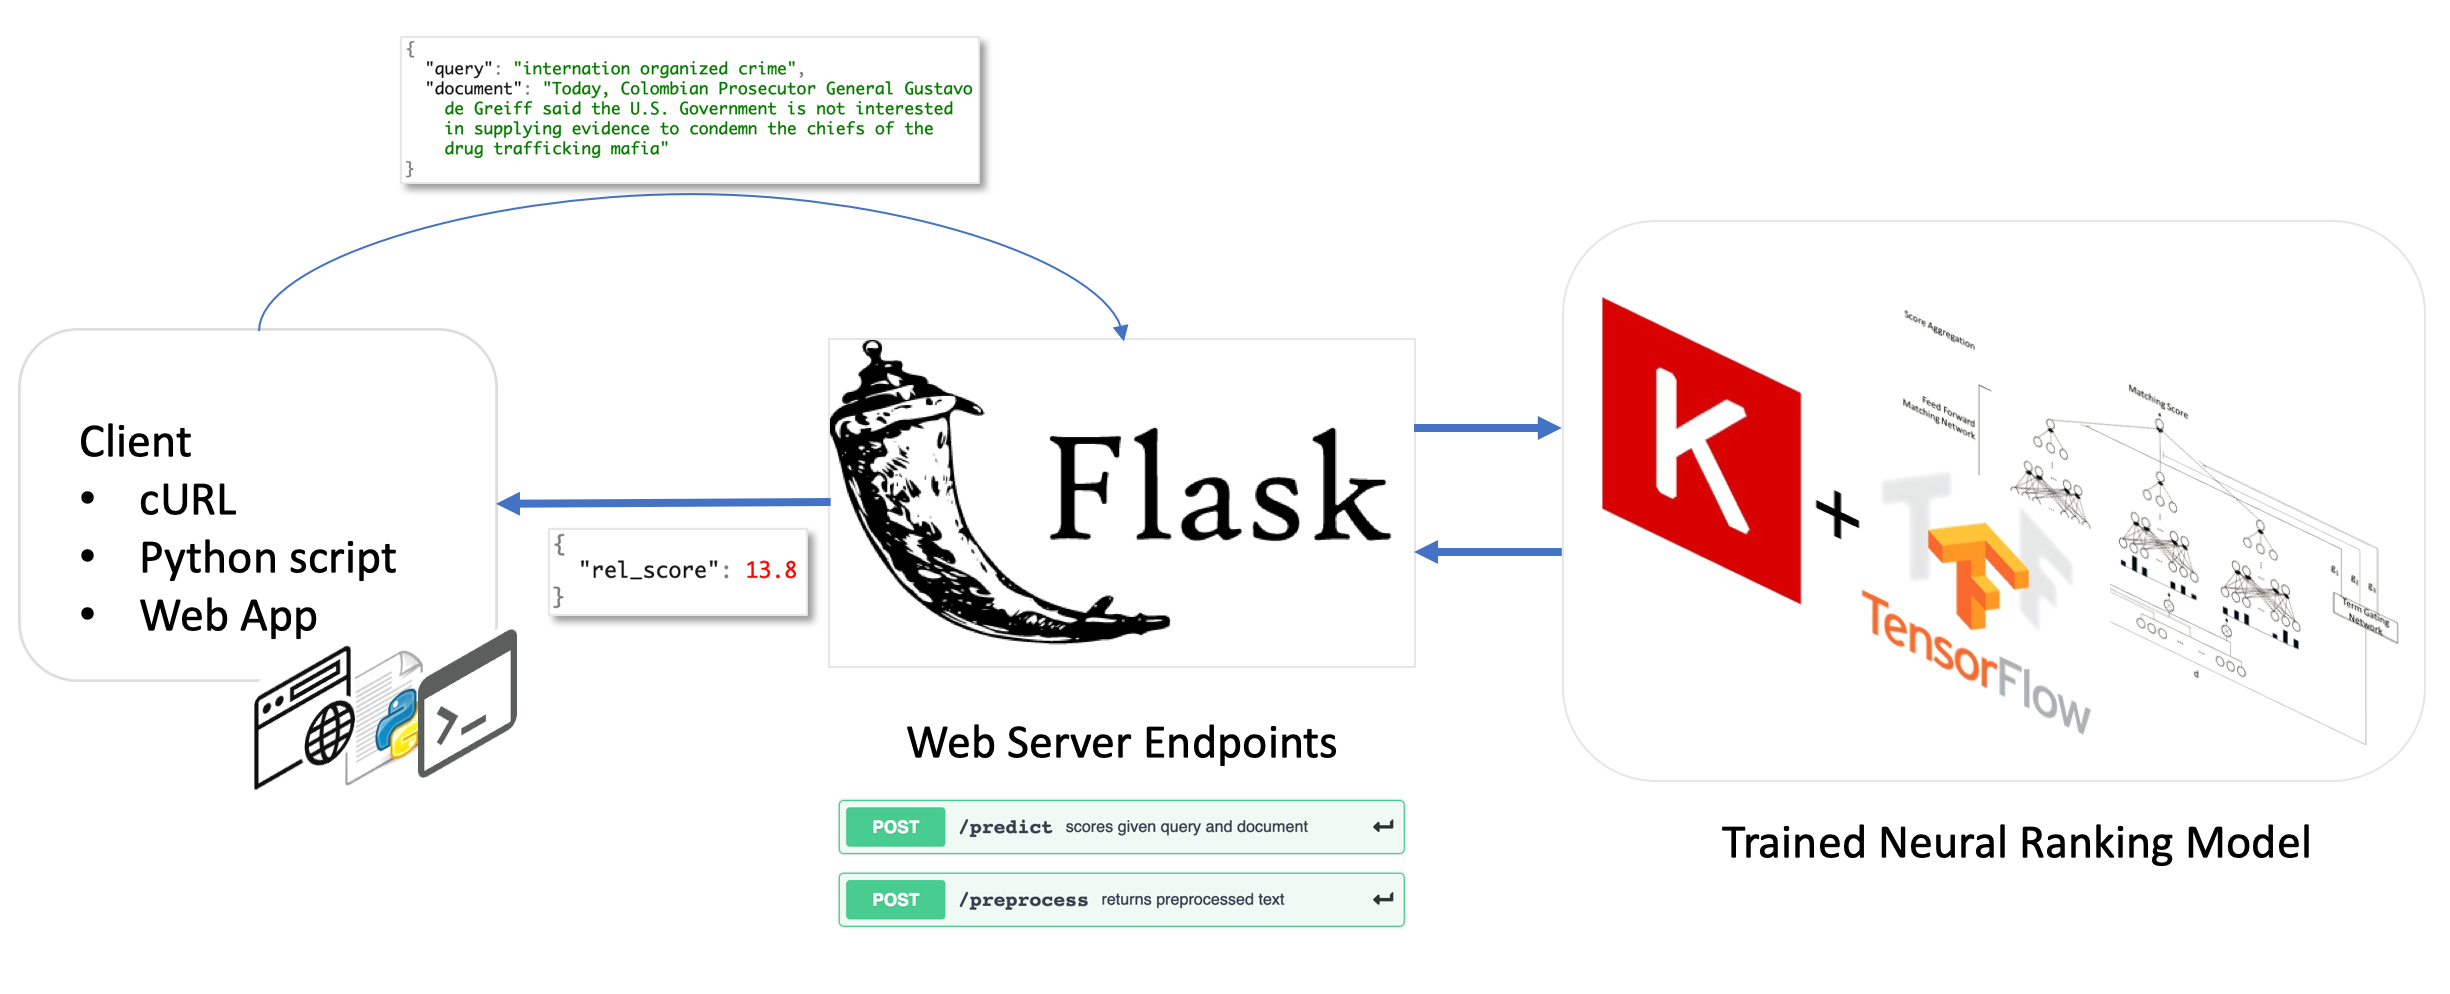
\includegraphics[width=\textwidth]{Figures/trained_model_deploy2.png}
    \caption{Deployment of NRMs workflow}
    \label{fig:nrm_deployment}
\end{figure}
% \clearpage
We have deployed some of the trained models (DRMM, MP-COS, PACRR-DRMM, NPRF\textsubscript{ds}-DRMM) using the Flask\footnote{\url{http://flask.pocoo.org/}} web framework. The Flask server first loads the pretrained Keras model that shows the best performance on MAP for Robust04 and exposes two REST API endpoints--for scoring a given query-document pair and for preprocessing the given text into the input format required by the pretrained model. The work flow of how the models are deployed is displayed in Figure.~\ref{fig:nrm_deployment}.

The endpoint for scoring can be used by any system that has a \textit{telescoping} setup that has to re-rank the initial set of retrieved documents (e.g. BM25 or QL) using one of the trained models. The second endpoint for preprocessing the given text is useful for interpretable visualizations such as heatmaps that highlights words in the document that are relevant/irrelevant to the query.
